%arara: lualatex: { branch: developer, interaction: errorstopmode,
%arara: --> shell: yes, synctex: yes }
%arara: makeglossaries if found('aux', '@istfilename')
%arara: biber: { options: [ '--wraplines' ] }

% \DocumentMetadata{testphase=phase-III}
% \DocumentMetadata{lang=es-MX}

% NOTA: [<+->] se usa comio overlay para hacer que los bullets aparezcan uno por uno.

\documentclass[spanish,mexico,12pt]{scrartcl}
% \listfiles

\KOMAoptions{abstract=true}
\usepackage[spanish,mexico]{babel}


\usepackage{fontspec}
    \setmainfont{TeX Gyre Pagella}
    \setsansfont{TeX Gyre Heros}

\renewcommand{\familydefault}{\sfdefault} % Sans serif

\usepackage{csquotes}
% \MakeAutoQuote{"}{"}

\usepackage{microtype}
\setlength{\parskip}{1em}
\usepackage{tabularray}
\UseTblrLibrary{booktabs}
\UseTblrLibrary{siunitx}

\usepackage{siunitx}
\sisetup{separate-uncertainty,per-mode=symbol,detect-all,range-phrase=--}
\DeclareSIUnit{\angstrom}{\textup{\AA}}
\usepackage{chemmacros}
\usepackage{glossaries}
    \makeglossaries{}

\usepackage[style=science,backend=biber,url=false]{biblatex}
    \addbibresource[location=remote]{http://127.0.0.1:23119/better-bibtex/export/library?/1/library.biblatex}

\usepackage[skins]{tcolorbox}
\usepackage{paralist}
\usepackage{cleveref}
\usepackage{subcaption}
\usepackage[colorinlistoftodos]{todonotes}
\usepackage{lineno}
\usepackage{rotating}
\usepackage{newfloat}
\DeclareFloatingEnvironment[
   fileext=los,
   listname={List of Schemes},
   name=Scheme,
   placement=tbp,
   within=none % don't reset numbering
]{scheme}
\DeclareCaptionSubType{scheme}
\setcounter{secnumdepth}{5}

\begin{filecontents}[force]{abreviaturas.tex}
    \newacronym{DFT}{DFT}{Teoría del funcional de la densidad \textit{(del inglés "Density Functional Theory")}}
    \newacronym{TDDFT}{TDDFT}{Teoría del funcional de la densidad tiempo-dependiente \textit{(del inglés "Time-Dependant Density Functional Theory")}}
    \newacronym{FMR}{FMR}{Rotores Moleculares Fluorescentes \textit{(Del inglés Flurescent Molecular Rotor)}}
    \newacronym{BOSCHIBA}{BOSCHIBA}{Bases de Schiff de Boro \textit{(del inglés "\textsc{Bo}ron \textsc{Schi}ff \textsc{Ba}ses")}}
    \newacronym{BODIPY}{BODIPY}{\textsc{bo}ron-\textsc{di}\textsc{py}rromethene}
    \newacronym{TICT}{TICT}{transferencia de carga intramolecular retorcida \textit{(del inglés "twsited intramolecular charge transfer")}}
    \newacronym{LE}{LE}{Local Excitado \textit{(del inglés "locally exited")}}
    \newacronym{MW}{MW}{Microondas \textit{(del inglés "Microwave")}}
    \newacronym{PES}{PES}{Superficie de Energía Potencial \textit{(del inglés "Potential Energy Surface")}}
    \newacronym{NBO}{NBO}{Orbitales Naturales de Enlace \textit{(del inglés "Natural Bond Orbitals")}}
    \newacronym{ICT}{ICT}{Transferencia de Carga Intramolecular \textit{(del inglés "Intramolecular Charge Transfer")}}
    \newacronym{VEE}{VEE}{Energía de Emisión Vertical \textit{(del inglés "Vertical Emission Energy")}}
    \newacronym{FMO}{FMO}{Orbitales Moleculares de Frontera \textit{(del inglés "Frontier Molecular Orbitals")}}
    \newacronym{HOMO}{HOMO}{Orbital Molecular de mas alta energía \textit{(del inglés "Highest Occupied Molecular Orbital")}}
    \newacronym{LUMO}{LUMO}{Orbital Molecular no ocupado de más baja energía \textit{(del inglés "Lowest Unoccupied Molecular Orbital")}}
    \newacronym{NMR}{NMR}{Resonancia Magnética Nuclear \textit{(del inglés "Nuclear Magnetic Resonance")}}
    \newacronym{CREST}{CREST}{\textit{Conformer-Rotamer Ensemble Sampling Tool}}
\end{filecontents}

\begin{filecontents}[force]{comandos.tex}
    % \newcommand{\invitro}{\textit{in-vitro}}
    \newcommand\scan{\(\text{r}^{2}\text{SCAN-3c}\)}
\end{filecontents}

\begin{filecontents}[force]{gantt.tex}
    \def\pgfcalendarweekdayletter#1{% \ifcase#1M\or T\or W\or T\or F\or S\or S\fi%
}
\begin{ganttchart}[
hgrid,
  vgrid,
  x unit=18mm,
  time slot format=little-endian
]{7.1.2013}{13.1.2013}
\gantttitlecalendar*{7.1.2013}{13.1.2013}{
month, month=name, month=shortname, weekday,
    weekday=name, weekday=shortname, weekday=letter
  }
\end{ganttchart}
\end{filecontents}

\begin{filecontents}[force]{quimica.tex}
    \DeclareChemReactant{BO-gly}{name={BO-Gly}} % 1
    \DeclareChemReactant{BO-trp}{name={BO-Trp}} % 2
    \DeclareChemReactant{BO-tyr}{name={Bo-Tyr}} % 3
    \DeclareChemReactant{BO-phe}{name={BO-Phe}} % 4
    \DeclareChemReactant{trp}{name={\iupac{\laevus-triptófano}}, short={trp}}
    \DeclareChemReactant{phe}{name={\iupac{\laevus-fenilalanina}}, short={phe}}
    \DeclareChemReactant{tyr}{name={\iupac{\laevus-tirosina}}, short={tyr}}
    \DeclareChemReactant{gly}{name={glicina}, short={gly}}
    \DeclareChemReactant{aphb}{name={ácido fenil borinico}, short={\ch{PhB(OH)2}}}
    \DeclareChemReactant{2h1n}{name={\iupac{2-Hidroxi-1-naftaldehido}}, short={\iupac{2-Hidroxi-1-naftaldehido}}}
    \NewChemLatin\invitro{in vitro}
    \NewChemLatin\invivo{in vivo}
    \NewChemLatin\insilico{in silico}
    \DeclareChemTranslation{scheme-name}{spanish}{Esquema}
    \DeclareChemTranslation{scheme-list}{spanish}{Lista de esquemas}
    \DeclareChemTranslation{scheme}{spanish}{esquema}
    \DeclareChemTranslation{schemes}{spanish}{esquemas}
    \DeclareChemTranslation{Scheme}{spanish}{Esquema}
    \DeclareChemTranslation{Schemes}{spanish}{Esquemas}
    \renewcommand{\schemename}{Esquema}
\end{filecontents}

%% LaTeX2e file `abreviaturas.tex'
%% generated by the `filecontents' environment
%% from source `PEAG-Protocolo_maestria' on 2023/09/17.
%%
    \newacronym{DFT}{DFT}{Teoría del funcional de la densidad \textit{(del inglés "Density Functional Theory")}}
    \newacronym{TDDFT}{TDDFT}{Teoría del funcional de la densidad tiempo-dependiente \textit{(del inglés "Time-Dependant Density Functional Theory")}}
    \newacronym{FMR}{FMR}{Rotores Moleculares Fluorescentes \textit{(Del inglés Flurescent Molecular Rotor)}}
    \newacronym{BOSCHIBA}{BOSCHIBA}{Bases de Schiff de Boro \textit{(del inglés "\textsc{Bo}ron \textsc{Schi}ff \textsc{Ba}ses")}}
    \newacronym{BODIPY}{BODIPY}{\textsc{bo}ron-\textsc{di}\textsc{py}rromethene}
    \newacronym{TICT}{TICT}{transferencia de carga intramolecular retorcida \textit{(del inglés "twsited intramolecular charge transfer")}}
    \newacronym{LE}{LE}{local excitado \textit{(del inglés "locally exited")}}

%% LaTeX2e file `comandos.tex'
%% generated by the `filecontents' environment
%% from source `Presentación-Protocolo-Maestria-PEAG' on 2023/11/14.
%%
    % \newcommand{\invitro}{\textit{in-vitro}}
    \newcommand\scan{\(\text{r}^{2}\text{SCAN-3c}\)}


%% LaTeX2e file `quimica.tex'
%% generated by the `filecontents' environment
%% from source `PEAG-Protocolo_maestria' on 2023/09/17.
%%
    \DeclareChemReactant{BO1}{name={BO1}, short={THF}}
    \DeclareChemReactant{BO-trp}{name={triptófano}, short={BO-trp}}
    \DeclareChemReactant{BO-phe}{name={fenilalanina}, short={BO-phe}}
    \DeclareChemReactant{BO-tyr}{name={tirosina}, short={BO-tyr}}
    \DeclareChemReactant{BO-gly}{name={glicina}, short={BO-gly}}
    \NewChemLatin\invitro{in vitro}
    \NewChemLatin\insilico{in silico}
    \DeclareChemTranslation{scheme-name}{spanish}{Esquema}
    \DeclareChemTranslation{scheme-list}{spanish}{Lista de esquemas}
    \DeclareChemTranslation{scheme}{spanish}{esquema}
    \DeclareChemTranslation{schemes}{spanish}{esquemas}
    \DeclareChemTranslation{Scheme}{spanish}{Esquema}
    \DeclareChemTranslation{Schemes}{spanish}{Esquemas}
    \renewcommand{\schemename}{Esquema}


\title{Síntesis sustentable, caracterización química-fotofísica, y por {DFT} de {BOSCHIBA} derivadas de aminoácidos y su aplicación \invitro{}}
\subject{Protocolo de tesis de maestría}
\date{\today}
\author{Pablo E. Alanis González}
\publishers{Universidad Autónoma de Nuevo León, División de Posgrado}

\begin{document}
% \linenumbers{}
\pagenumbering{roman}
\maketitle

\begin{abstract}
    Se sintetizarán una serie de \gls{BOSCHIBA} derivadas de \reactant*{gly}, \reactant*{trp}, \reactant*{tyr} y \reactant*{phe}. Se caracterizarán por métodos espectroscópicos y se realizarán cálculos \insilico{} por medio de \gls{DFT} y \gls{TDDFT} para estudiar las propiedades fotofísicas de los compuestos y comprobar los mecanismos involucrados en el efecto supresor de la luminiscencia en dichos compuestos así como estudios de topológicos sobre estos. A su vez, se realizarán estudios de citotoxicidad y tinción \invitro{} para determinar su actividad biológica de los compuestos.
\end{abstract}

\newpage
\vspace*{\fill}
\begin{tblr}{%
        colspec = {X[1,l,m] X[1,l,m]},
        % row{1} = {font=\bfseries}
    }
    \textbf{No. de folio}                                             & 03-97179QMT-23-107                                                \\
    \textbf{Programa academico}                                       & Maestría en Ciencias con orientación en química de los materiales \\
    \textbf{Línea de Generación y Aplicación del Conocimiento (LGAC)} & Materiales moleculares                                            \\
    \textbf{Lugar de realización}                                     & Facultad de Ciencias Químicas, UANL
\end{tblr}

\vspace{5cm}

\begin{tblr}{
        colspec = {X[1,r,m] X[2,l,m]},
        width = 0.7\linewidth
    }
    Aprueba: & \hrulefill                      \\
             & Dr. Víctor Manuel Jiménez Pérez \\
             & Director de tesis               \\
\end{tblr}

% \begin{tabular}{@{}p{1in}p{3in}@{}}
%     Aprueba: & \hrulefill                      \\
%              & Dr. Víctor Manuel Jiménez Pérez \\
%              & Director de tesis               \\
% \end{tabular}
\vspace*{\fill}
\newpage

\tableofcontents
\listoffigures
\listoftables
\listofschemes

\cleardoublepage
\pagenumbering{arabic}

\section{Introducción}

Recientemente, se ha acrecentado el interés por los compuestos fluorescentes de boro debido a su amplio campo de aplicaciones; \autocite{ibarra-rodriguezOrganoboronSchiffBases2019} ya sea en sensores, como en tintas de seguridad, o bien los \gls{BODIPY} comercialmente disponibles utilizados como agentes para la tinción celular, ER-Tracker™ Green y ER-Tracker™ Red (ver \cref{ER-Trackers}).

\begin{scheme}
    \centering
    \begin{subscheme}{0.45\linewidth}
        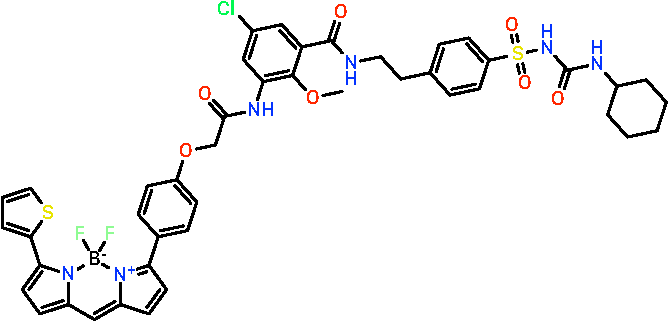
\includegraphics[width=\linewidth]{ER-Tracker_Blue.pdf}
        \caption{ER-Tracker™ Blue}
        \label{ER-Tracker_Blue}
    \end{subscheme}
    \hfill
    \begin{subscheme}{0.45\linewidth}
        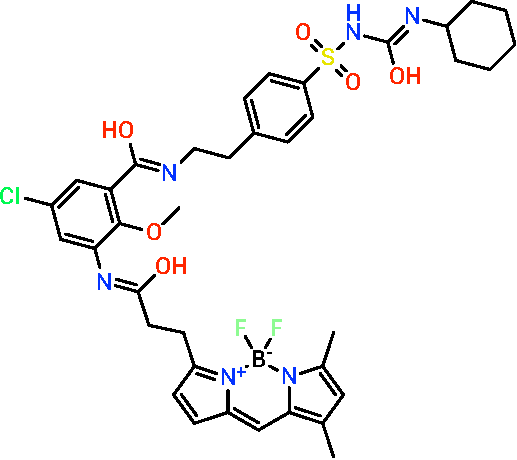
\includegraphics[width=\linewidth]{ER-Tracker_Green.pdf}
        \caption{ER-Tracker™ Green}
        \label{ER-Tracker_Green}
    \end{subscheme}
    \caption[ER-Trackers™]{Los ER-Tracker™ Green y ER-Tracker™ Red de Thermo Fischer Scientific™ son \gls{BODIPY} comerciales utilizados como agentes para la tinción celular.}
    \label{ER-Trackers}
\end{scheme}

Los \gls{FMR} son fluoróforos sensibles a la viscosidad que presentan una rotación libre que se vuelven fluorescentes, o en su defecto, aumentan la fluorescencia solo si su rotación se ve restringida.\todo{Citar} Algunas interacciones de carácter intramolecular para detener la rotación de los \gls{FMR} son \begin{inparaenum}[i.]
    \item formar interacciones de hidrógeno,\autocite{wuMultistageRotationalSpeed2018}
    \item a través del impedimento estérico,\autocite{faulknerAllostericRegulationRotational2016} o
    \item por la formación de complejos estables con iones metálicos.\autocite{yadavViscochromicMechanochromicUnsymmetrical2019}
\end{inparaenum}

Se ha determinado que la polarización del solvente y la viscosidad del mismo afectan considerablemente la fluorescencia de los \gls{FMR}. Esto es porque se limita la tasa de formación del complejo \gls{TICT}, el cual se de-exita de forma \emph{no-radiativa,} y se promueve la formación del complejo \gls{LE}, el cual fluórese. El efecto que tiene la polarización del solvente, aunque se sabe que es importante, no se ha logrado elucidar de forma aislada a la viscosidad.\cite{haidekkerEffectsSolventPolarity2005}

Diferentes estrategias para el diseño de \gls{FMR} se han propuesto para realizar sensores de viscosidad altamente sensibles, por ejemplo, incorporando grupos rotacionales asimétricos,\autocite{leePyrrolicMolecularRotors2016} rotadores con alta capacidad rotacional,\autocite{karpenkoPushPullDioxaborine2016} variación de puentes π-conjugados \emph{push-pull},\autocite{karpenkoPushPullDioxaborine2016} la aplicación de rotadores di- o trímeros,\autocite{kimballBODIPYBODIPYDyad2015} y la introducción de dos rotadores con diferentes capacidades rotacionales y electrondonantes.\autocite{rautTriazinebasedBODIPYTrimer2016}

Por lo que, obtener tanto una alta eficiencia de fluorescencia como un contraste fluorescente simultáneamente es muy difícil, debido a que, en muchos casos, las moléculas de alto rendimiento cuántico tienen una capacidad de contraste deficiente.
El rendimiento cuántico y el contraste de fluorescencia de los \gls{FMR} están inversamente correlacionados, una relación llamada "intensidad de fluorescencia---contraste".\autocite{leeFrontCoverFluorescent2018}

En la actualidad existe una amplia variedad de \gls{FMR} derivados de compuestos de boro, donde los \gls{BODIPY} y los dioxaborinos son los protagonistas debido a su elevado rendimiento cuántico, sin embargo, muestran algunas desventajas como la síntesis en varias etapas, condiciones de atmósfera anhidra y, en muchas ocasiones, una capacidad de contraste baja, aumentando escasamente el rendimiento cuántico del valor inicial.\autocite{karpenkoPushPullDioxaborine2016,guptaBodipyBasedFluorescent2016,liBODIPYBasedTwoPhotonFluorescent2018,kimBorondifluorideComplexesHemicurcuminoids2016}

Recientemente, nuestro grupo de trabajo ha informado sobre la síntesis de \gls{BOSCHIBA} y su uso como \gls{FMR} en la detección de viscosidad y la bioimagen de células.\autocite{ibarra-rodriguezFluorescentMolecularRotors2017} Los resultados encontrados indican que los \gls{BOSCHIBA} pueden aumentar hasta 34 veces su valor de rendimiento cuántico en medios de alta viscosidad, sin embargo, a pesar de teñir selectivamente el citoplasma en las células de melanoma, presentaron un bajo teñido atribuido principalmente a la baja solubilidad de los compuestos.

Para lograr mejorar el contraste de fluorescencia y la bioimagen celular, se diseñó una serie de \gls{BOSCHIBA} derivados de aminoácidos (ver \cref{sch:marcha}), donde las moléculas presentan rotación libre a través del anillo fenilborónico, y el aminoácido podría dar una mayor compatibilidad y solubilidad en medios celulares. Los compuestos de boro fluorescentes \textbf{1-4} se obtuvieron por irradiación ultrasónica en combinación con una reacción multicomponente con altos rendimientos químicos (\qty{>90}{\percent}) y un tiempo de reacción corto de \qty{20}{\minute} a \qty{50}{\degreeCelsius}. Este método resulta más eficiente y rápido en comparación con moléculas similares reportadas en la literatura.

\begin{scheme}
    \centering
    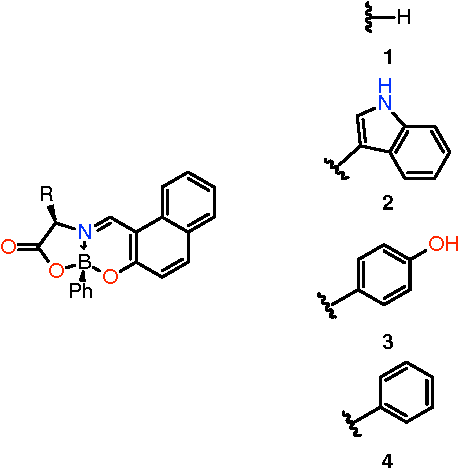
\includegraphics[width=0.5\linewidth]{Marcha.pdf}
    \caption{Compuestos que se sintetizarán en esta investigación.}
    \label{sch:marcha}
\end{scheme}

\section{Antecedentes}
\SetTblrInner{fontsize}{\fontsize{10}{12}\selectfont}
\begin{longtblr}[
        caption={Antecedentes de la investigación.},
        label={tbl:antecedentes}
    ]{
        colspec = {X[2,c,m] X[2,c,m] X[c,m]},
        % rowhead = 1,
        cells   = {font = \fontsize{8pt}{10pt}\selectfont},
        row{1} = {font=\bfseries}
    }
    \toprule
    Investigación                                                       & Aportación(es)                                                                   & Referencia                                                    \\ \midrule
    \citetitle*{lopez-espejelOrganotinSchiffBases2021}                  & Sintesis por \gls{MW} de \gls{BOSCHIBA} con \ch{Sn}                                           & \cite{lopez-espejelOrganotinSchiffBases2021}                  \\
    \citetitle*{garcia-lopezNewLuminescentOrganoboron2022}              & Síntesis de \gls{BOSCHIBA} por reacción \textit{one-pot} multicomponente (3-MCR) & \cite{garcia-lopezNewLuminescentOrganoboron2022}              \\
    \citetitle*{corona-lopezFarRedInfrared2021}                         & Síntesis de \gls{BOSCHIBA} con clusters de boro                                  & \cite{corona-lopezFarRedInfrared2021}                         \\
    \citetitle*{ibarra-rodriguezOrganoboronSchiffBases2019}             & Síntesis de \gls{BOSCHIBA} y su uso como sondas fluorescentes                    & \cite{ibarra-rodriguezOrganoboronSchiffBases2019}             \\
    \citetitle*{canton-diazOnepotMicrowaveassistedSynthesis2018}        & Sintesis \textit{one-pot} de \gls{BOSCHIBA}                                      & \cite{canton-diazOnepotMicrowaveassistedSynthesis2018}        \\
    \citetitle*{corona-lopezSynthesisCharacterizationPhotophysical2017} & Síntesis de \gls{BOSCHIBA} y su aplicación para teñir citoplasma                 & \cite{corona-lopezSynthesisCharacterizationPhotophysical2017} \\
    \bottomrule
\end{longtblr}

\subsection{Análisis crítico de los antecedentes}

\textcite{ibarra-rodriguezOrganoboronSchiffBases2019} investigaron la aplicación de \gls{BOSCHIBA} en fluorescencia y bioimagen celular. Por su respuesta a la viscosidad, resultante en un aumento en el rendimiento cuántico, se propuso su uso para detección de células cancerígenas. Los autores mencionan que es importante para diseñar marcadores citoplasmáticos que sean fluorescentes, con propiedades fotofísicas adecuadas, fotoestables, con baja citotoxicidad y solubles en solventes polares para ser usados en biología celular moderna \invitro{} y \invivo{}; en esta investigación se lograron teñir las células cancerígenas B16F10, sin embargo, el teñido del citoplasma fue bajo, atribuido principalmente a la baja solubilidad de los compuestos; por lo que en esta investigación se propone la síntesis de \gls{BOSCHIBA} derivada de aminoácidos, con el fin de mejorar la solubilidad de los compuestos y lograr un mejor teñido del citoplasma.

\textcite{corona-lopezFarRedInfrared2021} propone la preparación de \gls{BOSCHIBA} a partir de la condensación de \reactant{2h1n} con la amina correspondiente; en esta investigación obtuvieron buenos rendimientos  (\qtyrange{85}{90}{\percent}), sin embargo el tiempo de reacción fue de \qty{48}{\hour}, por lo que llevar a cabo esta síntesis por medio de \gls{MW} en lugar de por reflujo convencional podría resultar en un menor tiempo de reacción.

El estudio realizado por \textcite{garcia-lopezNewLuminescentOrganoboron2022} detalla la síntesis de \gls{BOSCHIBA} tetracoordinados vía una reacción de condensación de tres componentes con rendimientos elevados \qtyrange{80}{90}{\percent} en un tiempo de reacción de \qty{20}{\minute}.

En una investigación donde se preparan bases de Schiff basadas en \ch{Sn} realizada por \textcite{lopez-espejelOrganotinSchiffBases2021} se conduce la reacción por medios convencionales de calentamiento y por \gls{MW}; el tiempo de reacción se vio drásticamente reducido, de \qty{24}{\hour} a \qty{3}{\minute}, y los rendimientos mejoraron. En este estudio también se evaluó el uso de bases de Schiff basadas en \ch{Sn} como agentes de tinción celular y se encontró que tienen baja citotoxicidad y buena capacidad de tinción.



\section{Aportación científica}
Plantear una metodología para la sintesis de compuestos de boro fluorescentes, con un alto rendimiento cuántico y un alto contraste de fluorescencia en medios de alta viscosidad, a partir de aminoácidos, así como su aplicación en la bioimagen de células. También se realizarán estudios \insilico{} para determinar las propiedades fotofísicas de los compuestos.

\section{Hipótesis}
La incorporación de aminoácidos en la estructura de los \gls{BOSCHIBA} logrará una mejor penetración de las membranas celulares, además de que se espera que los compuestos presenten un alto rendimiento cuántico y un alto contraste de fluorescencia en medios de alta viscosidad.

\section{Objetivos y metas}
\subsection{Objetivo general}
Realizar la síntesis de una serie de \gls{BOSCHIBA} con su posible aplicación en tinción celular y estudiar sus propiedades fotofísicas por medio de cálculos \insilico{}.

\subsection{Objetivos específicos}
\begin{itemize}
    \item \textbf{Sintetizar} una serie de \gls{BOSCHIBA} derivadas de \reactant{trp}, \reactant{phe}, \reactant{tyr} y \reactant{gly};
    \item \textbf{Elucidar} los mecanismos involucrados en el efecto supresor de la luminiscencia en \reactant{BO-trp};
    \item \textbf{Caracterizar} los compuestos por métodos espectroscópicos;
\end{itemize}

\section{Metodología}
\subsection{Materiales}
\begin{longtblr}[
        caption = {Equipos que se utilizarán para la caracterización de los compuestos de esta investigación.},
        entry = {Instrumentos de caracterización.},
        label = {tbl:equipos}
    ]{
        colspec = {X[2,c,m] X[c,m] X[c,m]},
    }
    \toprule
    \textbf{Instrumento}                             & \textbf{ Marca y modelo} & \textbf{Locación}          \\ \midrule
    Espectrofotómetro                                & {Perkin-Elmer,                                        \\Lambda 365} & FCQ \\
    Espectrofluorímetro                              & {Horriba Scientificm,                                 \\Fluorolog-3} & FCQ \\
    Sistema LC/MS/MS                                 & {EMAR,                                                \\AB Sciex API 2000} & CINVESTAV---IPN (DF) \\
    Difractómetro de rayos X                         & {Bruker,                                              \\SMART APEX CCD} & CINVESTAV---IPN (DF) \\
    \gls{NMR} (\NMR*{1,H}, \NMR*{11,B}, \NMR*{13,C}) & {Bruker,                                              \\Avance DPX 400} & Facultad de Medicina, UANL \\
    Microscopio confocal                             & ---                      & Facultad de Biología, UANL \\
    \bottomrule
\end{longtblr}

\subsection{Experimental}
\subsubsection{Síntesis}
Se llevará acabo la síntesis de los compuestos \textbf{1-4} (ver \cref{sch:marcha}) utilizando condiciones de reacción ecológicas y materiales de partida accesibles.
Se optimizarán los parámetros de reacción para obtener rendimientos elevados y selectividad adecuada.

\subsubsection{Determinación de propiedades ópticas}
Se determinará el rendimiento cuántico de los compuestos \textbf{1-4}, así como su contraste de fluorescencia en medios de viscosidad variable.

\subsubsection{Determinación de citotoxicidad}
Se determinará la citotoxicidad de los compuestos \textbf{1-4} en la línea celular de melanoma murino \emph{B16F10} (ATCC® CCL-6475™) derivado de ratón C57BL/6J.

\subsubsection{Modelado molecular}
Se realizarán cálculos \insilico{} por medio de \gls{DFT} y \gls{TDDFT} para estudiar las propiedades fotofísicas de los compuestos y comprobar los mecanismos involucrados en el efecto supresor de la luminiscencia en dichos compuestos así como estudios de topológicos sobre estos.

\paragraph{Preoptimización}
En caso de no contar con datos cristalográficos en el momento del estudio \insilico{}, se hará una búsqueda conformacional con ayuda del programa \gls{CREST} \cite{prachtAutomatedExplorationLowenergy2020} para obtener los conformeros más estables de los compuestos.

En caso de que se cuenten con datos cristalográficos, se utilizarán las coordenadas de la estructura cristalográfica para realizar la optimización geométrica en DFT.

\paragraph{Optimización geométrica}
Se hará la optimización geométrica de los compuestos \textbf{1-4} empleando el funcional meta-GGA \scan{}\footnote{La selección de este funcional para la optimización geométrica se debe a su desempeño comparable o superior con funcionales híbridos meta-GGA como M06-2X-D3(0)/TZP que costarían más tiempo de cómputo, así como su inclusión de correcciones relativistas como ECP y corrección para dispersión y su buen desempeño con el \emph{benchmark} LMGB35 (Enlaces ligeros del grupo principal) y ROT34 (constantes rotacionales de moléculas orgánicas pequeñas)} \cite{gasevicOptimizationSCAN3cComposite2022} hasta llegar a un nivel de teoría de DFT/def2-TZVP, o superior en caso de que sea necesario.

\paragraph{Obtención de espectro de emisión}
Se obtendrá el espectro de emisión de los compuestos \textbf{1-4} por medio de cálculos \gls{TDDFT} con el funcional ωB97X-V y con el fin de aproximarse al límite CBS, se requiere de aumentación con funciones difusas dobles, por lo que se usará el conjunto de funciones base def2-TZVPD o def2-QZVPPD si es necesario obtener estados de Rydberg.

\subsection{Disposición de resiudos}
\begin{longtblr}[
        caption = {Residuos que se generarán derivados de esta investigación.},
        entry = {Residuos.},
        label = {tbl:residuos}
    ]{
        colspec = {X[2,c,m] X[2,c,m] X[c,m]},
    }
    \toprule
    \textbf{Resiudo}  & \textbf{Tipo}                   & \textbf{Disposición} \\ \midrule
    \ch{MeOH}, hexano & Solventes orgánicos             & C                    \\
    DCM, Cloroformo   & Solventes orgánicos halogenados & C                    \\
    Sales inorgánicas & Sales                           & A                    \\
    \bottomrule
\end{longtblr}

\subsection{Costos}
Se estima un costo aproximado de \num{70000.00} MXN para la realización de esta investigación, el cual se desglosa en las \cref{tbl:costos-react,tbl:costos-caract}.

\subsubsection{Materiales}
El costo de los materiales para la preparación de las muestras y para el estudio \insilico{} no se incluye en el costo total de la investigación, ya que estos se encuentran disponibles en los laboratorios de la Facultad de Ciencias Químicas de la UANL y en el CINVESTAV.

\subsubsection{Reactivos}
Todos los reactivos en la \cref{tbl:costos-react} se adquirirán en la empresa Merck KGaA.

\begin{longtblr}[
        caption = {Costos de los reactivos. \textit{(Costos aproximados)}},
        entry = {Costos de los reactivos.},
        label = {tbl:costos-react}
    ]{
        colspec={X[2,c,m] X[1,c,m] X[1.5,c,m] X[1.5,c,m,si={table-format=4.2}]},
        % rowhead=1
    }
    \toprule
    \textbf{Reactivo} & CAS               & Cantidad         & \textbf{Costo total (MXN)} \\ \midrule
    \reactant{trp}    & \texttt{73-22-3}  & \qty{25}{\gram}  & 1017.00                    \\
    \reactant{phe}    & \texttt{63-91-2}  & \qty{25}{\gram}  & 971.00                     \\
    \reactant{tyr}    & \texttt{60-18-4}  & \qty{50}{\gram}  & 2223.00                    \\
    \reactant{gly}    & \texttt{56-40-6}  & \qty{500}{\gram} & 764.00                     \\
    \reactant{aphb}   & \texttt{98-80-6}  & \qty{50}{\gram}  & 2359.00                    \\
    \reactant{2h1n}   & \texttt{708-06-5} & \qty{100}{\gram} & 1769.00                    \\
    \midrule
    \textbf{Total}    &                   &                  & 9093.00                    \\
\end{longtblr}

\subsubsection{Métodos de caracterización}
\begin{longtblr}[
        caption = {Costos de los metodos de cacterización. \textit{(Costos aproximados)}},label={tbl:costos-caract},
        entry = {Costos de los metodos de cacterización.}
    ]{
        colspec={X[2,c,m] X[1,c,m] X[1.5,c,m,si={table-format=4.2}] X[1.5,c,m,si={table-format=4.2}]},
        % rowhead=1
    }
    \toprule
    \textbf{Análisis}   & Muestras & \textbf{Costo unitario (MXN)} & \textbf{Costo total (MXN)} \\ \midrule
    XRD                 & 4        & 800.00                        & 3200.00                    \\
    NMR                 & 4        & 2250.00                       & 9000.00                    \\
    FTIR                & 4        & 700.00                        & 2800.00                    \\
    UV-Vis              & 4        & 500.00                        & 2000.00                    \\
    LC/MC/MS            & 4        & 800.00                        & 3200.00                    \\
    Espectrofluorímetro & 4        & 500.00                        & 2000.00                    \\
    \midrule
    \textbf{Total}      &          &                               & 22200.00                   \\
\end{longtblr}

\begin{sidewaysfigure}
    \section{Planificación}
    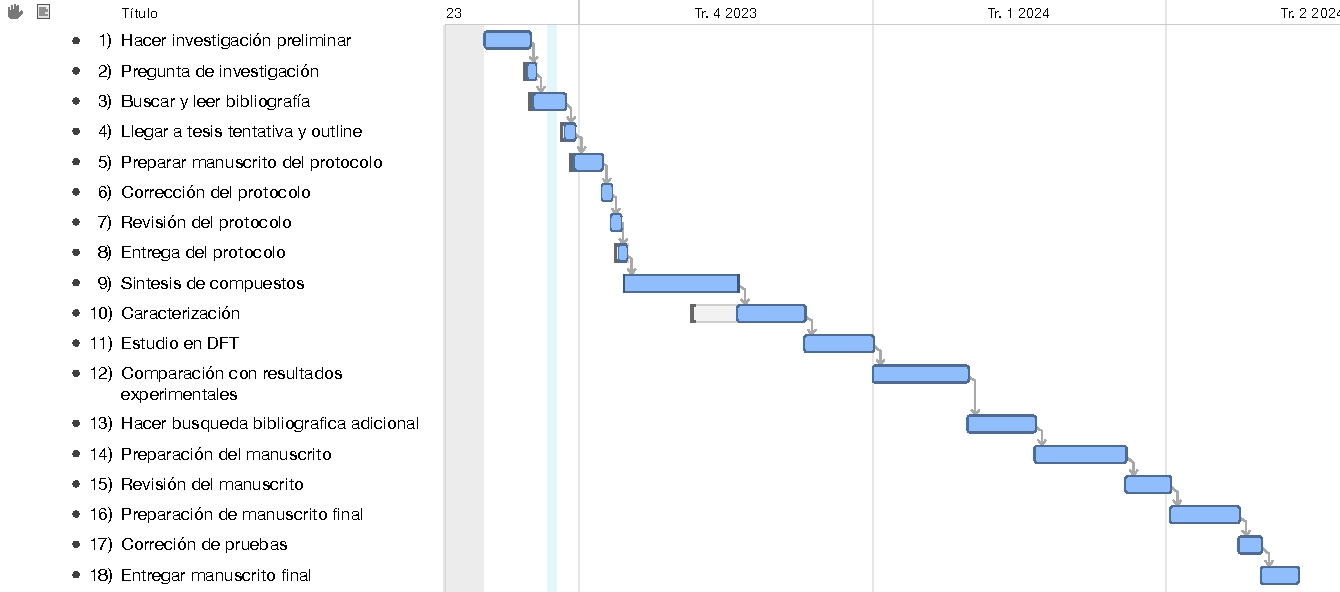
\includegraphics[width=0.9\linewidth]{gantt.pdf}
    \caption{Diagrama de Gantt de la investigación.}
    \label{fig:gantt}
\end{sidewaysfigure}
\printreactants{}
\printglossaries{}
\printbibliography{}

\listoftodos[Pendientes]

\end{document}
